% Figure 5.1 (Session 5): the Jordan-Wigner dictionary and its string.
% The image is rendered by figures/blender/s5_1_jw_string.py; the coordinates of the labels
% come from figures/blender/out/jw_string_anchors.tex. Built by figures/blender/build_figure.sh.
\documentclass[11pt,tikz,border=0pt]{standalone}
\usepackage{amsmath,amssymb,graphicx,braket}
\usepackage{xcolor}
\definecolor{coursedark}{HTML}{1B2A4A}
\definecolor{costamber}{HTML}{B8620A}
\definecolor{sviolet}{HTML}{6A3FC8}
\newlength{\figw}\setlength{\figw}{16.19cm}   % the text width of the notes (letter, 2.7 cm margins), so labels print at size

\begin{document}
\begin{tikzpicture}[lbl/.style={font=\small, text=coursedark}]
  \node[anchor=south west, inner sep=0pt] at (0,0)
    {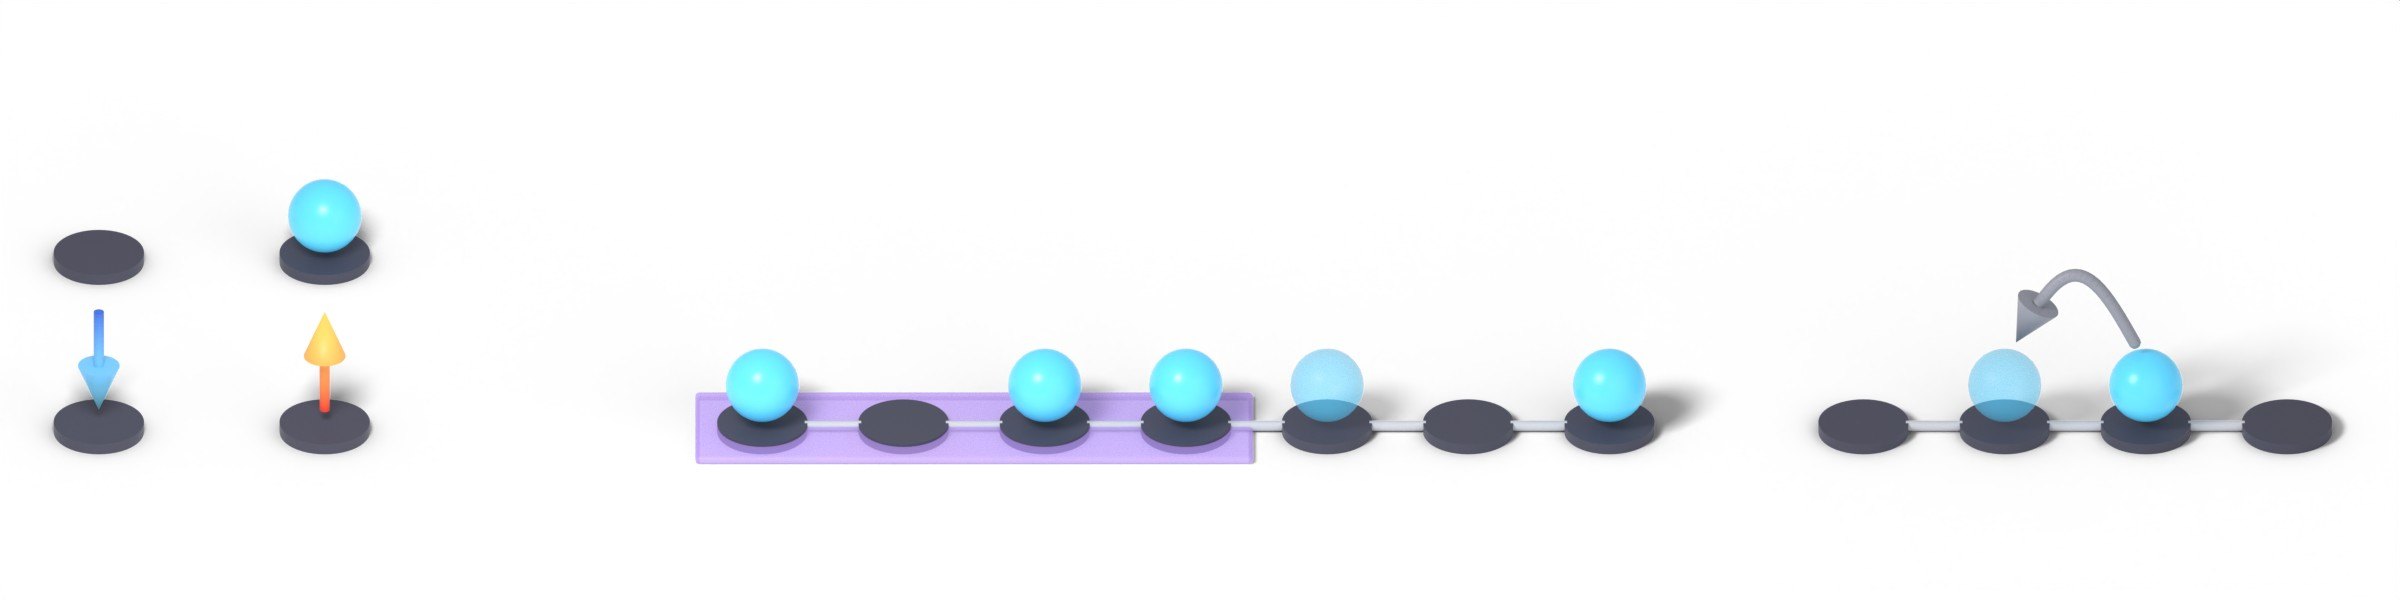
\includegraphics[width=\figw]{../blender/out/jw_string.jpg}};
  %% written by figlib.py; x and y in units of the image width
\coordinate (a) at (-0.0118\figw,0.2018\figw);
\coordinate (k0) at (0.0147\figw,0.1458\figw);
\coordinate (k1) at (0.1588\figw,0.1585\figw);
\coordinate (kdn) at (0.0176\figw,0.0956\figw);
\coordinate (kup) at (0.1588\figw,0.0956\figw);
\coordinate (match0) at (0.0412\figw,0.1123\figw);
\coordinate (match1) at (0.1353\figw,0.1123\figw);
\coordinate (p0) at (0.3176\figw,0.1236\figw);
\coordinate (p1) at (0.3765\figw,0.1236\figw);
\coordinate (p2) at (0.4353\figw,0.1236\figw);
\coordinate (p3) at (0.4941\figw,0.1236\figw);
\coordinate (ci) at (0.5529\figw,0.1236\figw);
\coordinate (ib) at (0.5529\figw,0.0554\figw);
\coordinate (Ki) at (0.3853\figw,0.0481\figw);
\coordinate (b) at (0.2765\figw,0.2018\figw);
\coordinate (hopc) at (0.8647\figw,0.1440\figw);
\coordinate (ic) at (0.8353\figw,0.0554\figw);
\coordinate (ic1) at (0.8941\figw,0.0554\figw);
\coordinate (one) at (0.8647\figw,0.0186\figw);
\coordinate (c) at (0.7353\figw,0.2018\figw);

  \node[lbl, font=\normalsize, anchor=west] at (a) {(a)};
  \node[lbl, font=\normalsize, anchor=west] at (b) {(b)};
  \node[lbl, font=\normalsize, anchor=west] at (c) {(c)};
  \node[lbl, anchor=east] at (k0) {$\ket{0}$};
  \node[lbl, anchor=west] at (k1) {$\ket{1}$};
  \node[lbl, anchor=east] at (kdn) {$\ket{\downarrow}$};
  \node[lbl, anchor=west] at (kup) {$\ket{\uparrow}$};
  \node[lbl, text=sviolet, anchor=south] at (p0) {$-1$};
  \node[lbl, text=sviolet, anchor=south] at (p1) {$+1$};
  \node[lbl, text=sviolet, anchor=south] at (p2) {$-1$};
  \node[lbl, text=sviolet, anchor=south] at (p3) {$-1$};
  \node[lbl, anchor=south] at (ci) {$c^\dagger_i$};
  \node[lbl, anchor=north] at (ib) {$i$};
  \node[lbl, text=sviolet, anchor=north] at (Ki) {$K_i=\prod_{j<i}(1-2n_j)=-1$};
  \node[lbl, anchor=south] at (hopc) {$c^\dagger_i c^{\phantom{\dagger}}_{i+1}$};
      \node[lbl, anchor=north east] at ([xshift=-0.05cm]ic) {$i$};
  \node[lbl, anchor=north west] at ([xshift=0.05cm]ic1) {$i+1$};
  \node[lbl, anchor=north] at (one) {$\prod_{i<k<i+1}(1-2n_k)=1$};
\end{tikzpicture}
\end{document}
